\newpage
\section{Statistical Survey Sampling}
\begin{figure*}[t]
\centering
\includegraphics[width=0.95\textwidth]{Images/SamplingDesign_\ldoc.png}
\caption[\small The sampling model]{\small Various populations and samples in the sampling model.} \hrule\label{fig:sammod}
\end{figure*}

\begin{tcolorbox}[title=You Can't Say It's Not True]
%Figures often beguile me, particularly when I have the arranging of them myself; in which case the remark attributed to Disraeli would often apply with justice and force: 'There are three kinds of lies: lies, damned lies, and statistics.' 
The latest survey shows that 3 out of 4 people make up 75\% of the world's population.\\[-0.6cm]
\begin{flushright}
%-- Mark Twain, \textit{Chapters of My Autobiography}, 1906
-- David Letterman (attributed)
\end{flushright}
\end{tcolorbox}
\noindent
While the \textit{World Wide Web} does contain troves of data, web scraping does not address the question of data validity: will the extracted data be \textbf{useful} as an analytical component? Will it  suffice to provide the quantitative answers that the client is seeking? 

A \textbf{survey} (a fair amount of information for this section is taken from \cite{DC_F,DC_SC}) is any activity that collects information about characteristics of interest:
\begin{itemize}[noitemsep] 
\item in an \textbf{organized} and \textbf{methodical} manner;
\item from some or all \textbf{units} of a population;
\item using \textbf{well-defined} concepts, methods, and procedures, and
\item compiles such information into a \textbf{meaningful} summary form. 
\end{itemize}
A \textbf{census} is a survey where information is collected from all units of a population, whereas a \textbf{sample survey} uses only a fraction of the units. 
%\afterpage{\FloatBarrier}
\subsection{Sampling Model}
When survey sampling is done properly, we may be able to use various statistical methods to make inferences about the \textbf{target population} by sampling a (comparatively) small number of units in the \textbf{study population}. The relationship between the various populations (\textbf{target}, \textbf{study}, \textbf{respondent}) and samples (\textbf{sample}, \textbf{intended}, \textbf{achieved}) is illustrated in Figure~\ref{fig:sammod}. 
\subsection{Deciding Factors} In some instances, information about the \textbf{entire} population is required in order to solve the client's problem, whereas in others it is not necessary.  How does one determine which type of survey must be conducted to collect data? The answer depends on multiple factors: 
\begin{itemize}[noitemsep]
    \item the type of question that needs to be answered;
\item the required precision;
\item the cost of surveying a unit;
\item the time required to survey a unit; \item size of the population under investigation, and 
\item the prevalence of the attributes of interest.
\end{itemize}
Once a choice has been made, each survey typically follows the same \textbf{general steps}:
\begin{enumerate}[noitemsep]
    \item statement of objective
    \item selection of survey frame
    \item sampling design
    \item questionnaire design
    \item data collection
    \item data capture and coding
    \item data processing and imputation
    \item estimation
    \item data analysis
    \item dissemination and  documentation
\end{enumerate}
The process is not always linear, in that preliminary planning and data collection may guide the implementation (selection of a frame and of a sampling design, questionnaire design), but there is a definite movement from objective to dissemination.   
\subsection{Survey Frames} The \textbf{frame} provides the means of \textbf{identifying} and \textbf{contacting} the units of the study population. It is generally costly to create and to maintain (in fact, there are organisations and companies that specialise in building and/or selling such frames). Useful frames contain: 
\begin{itemize}[noitemsep]
\item identification data, 
\item contact data, 
\item classification data,
\item maintenance data, and 
\item linkage data.
\end{itemize} The ideal frame must minimize the risk of \textbf{undercoverage} or \textbf{overcoverage}, as well as the number of \textbf{duplications} and \textbf{misclassifications} (although some issues that arise can be fixed at the data processing stage).\par Unless the selected frame is \textbf{relevant} (which is to say, it corresponds, and permits accessibility to, the target population), \textbf{accurate} (the information it contains is valid), \textbf{timely} (it is up-to-date), and \textbf{competitively priced}, the statistical sampling approach is contraindicated. 
\subsection{Survey Error} 
One of the strengths of statistical sampling is in its ability to provide estimates of various quantities of interest in the target population, and to provide some control over the  \textbf{total error} (TE) of the estimates. The TE of an estimate is the amount by which it differs from the true value for the target population:
\begin{align*} 
\TE  & =  \ME  +  \SaE \\ &\qquad +  \NE +  \CE, \end{align*}
where the 
\begin{itemize}[noitemsep]
\item \textbf{coverage error} is due to differences in the study and target populations; 
\item \textbf{non-response error} is due to differences in the respondent and study populations;
\item \textbf{sampling error} is due to differences in the achieved sample and the respondent population; 
\item \textbf{measurement error} is due to true value in the achieved sample not assessed correctly.
\end{itemize}
If we let 
\begin{itemize}[noitemsep]
\item $\overline{x}$ be the computed attribute value in the achieved sample; 
\item $\overline{x}_{\mathrm{true}}$ be the true attribute value in the achieved sample under perfect measurement;
\item $x_{\mathrm{resp}}$ be the attribute value in the respondent population;
\item $x_{\mathrm{study}}$ be the attribute value in the study population, and 
\item $x_{\mathrm{tar}}$ be the attribute value in the target population,
\end{itemize}
then 
\begin{align*}\TE  &= \overline{x} - x_{\mathrm{tar}} \\ & =  (\overline{x} - \overline{x}_{\mathrm{true}}) + (\overline{x}_{\mathrm{true}}-x_{\mathrm{resp}}) \\ &\qquad + (x_{\mathrm{resp}}-x_{\mathrm{study}}) + (x_{\mathrm{study}}-x_{\mathrm{tar}}).\end{align*} In an ideal scenario, $\TE=0$. In practice, there are two main contributions to $\TE$: \textbf{sampling errors} (which we will discuss shortly) and \textbf{nonsampling errors}, which include every contribution to survey error which is not due to the choice of sampling scheme. The latter can be controlled, to some extent: 
\begin{itemize}[noitemsep]
\item \textbf{coverage error} can be minimized by selecting a high quality, up-to-date survey frame;
\item \textbf{non-response error} can be minimized by careful choice of the data collection mode and questionnaire design, and by using ``call-backs'' and ``follow-ups'';
\item \textbf{measurement error} can be minimized by careful questionnaire design, pre-testing of the measurement apparatus, and cross-validation of answers.  
\end{itemize}
These suggestions are perhaps less useful than one could hope in modern times: survey frames based on landline telephones are quickly becoming irrelevant in light of an increasingly large and younger population who eschew such phones, for instance, while response rates for surveys that are not mandated by law are  surprisingly low. This explains, in part, the impetus towards automated data collection and the use of \textbf{non-probabilistic sampling} methods.     
\subsection{Modes of Data Collection}
How is data traditionally captured, then? There are \textbf{paper-based} approaches, \textbf{computer-assisted} approaches, and a suite of other modes.  
\begin{itemize}[noitemsep]
\item \textbf{Self-administered questionnaires} are used when the survey requires detailed information to allow the units to consult personal records (which reduces measurement errors), they are useful to measure responses to sensitive issues as they provide an extra layer of privacy, and are typically not as costly as other collection modes, but they tend to be associated with high non-response rate since there is less pressure to respond. 
\item \textbf{Interviewer-assisted questionnaires} use trained interviewers to  increase the response rate and overall quality of the data. Face-to-face \textbf{personal interviews} achieve the highest response rates, but they are costly (both in training and in salaries). Furthermore, the interviewer may be required to visit any selected respondents many times before contact is established. \textbf{Telephone interviews}, on the other hand produce ``reasonable'' response rates at a reasonable cost and they are safer for the interviewers, but they are limited in length due to respondent phone fatigue. With random dialing, 4-6 minutes of the interviewer's time is spent in out-of-scope numbers for each completed interview.
\item \textbf{Com\-puter-assisted interviews} combine data collection and data capture, which saves valuable time, but the drawback is that not every sampling unit may have access to a computer/data recorder (although this is becomine less prevalent). All paper-based modes have a computer-assisted equivalent: \textbf{com\-puter-as\-sisted self-interview} (CASI), \textbf{com\-puter-as\-sisted interview} (CAI),  \textbf{com\-puter-as\-sisted tele\-phone interview} (CATI), and 
\textbf{com\-puter-as\-sisted personal interview} (CAPI).
\item Unobtrusive direct observation
\item Diaries to be filled (paper or electronic)
\item Omnibus surveys
\item Email, Internet, and social media
\end{itemize}
\subsection{Non-Probabilistic Sampling}
There exists a number of methods to select sampling units from the target population that use subjective, non-random approaches (NPS). These methods tend to be \textbf{quick}, \textbf{relatively inexpensive} and \textbf{convenient} in that a survey frame is not needed. NPS methods are ideal for \textbf{exploratory analysis} and \textbf{survey development}. \newl Unfortunately, they are sometimes used \textbf{instead} of probabilistic sampling designs, which is problematic; the associated selection bias makes NPS methods \textbf{unsound} when it comes to \textbf{inferences}, as they cannot be used to provide \textbf{reliable estimates of the sampling error} (the only component of $\TE$ on which the analysts has direct control). Automated data collection often fall squarely in the NPS camp, for instance. While we can still analyse data collected with a NPS approach, we \textbf{may not generalise the results} to the target  population (except in rare, census-like situations). \newl
NPS methods include
\begin{itemize}[noitemsep]
\item \textbf{Haphazard} sampling, also known as `man on the street' sampling; it assumes that the population is homogeneous, but the selection remains subject to interviewer biases and the availability of units;
\item \textbf{Volunteer} sampling in which the  respondents are self-selected; there is a large selection bias since the silent majority does not usually volunteer; this method is often imposed upon analysts due to ethical considerations; it is also used for focus groups or qualitative testing;
\item \textbf{Judgement} sampling is based on the analysts' ideas of the target population composition
 and behaviour (sometimes using a prior study); the units are selected by population experts, but inaccurate preconceptions can introduce large biases in the study;
\item \textbf{Quota} sampling is very common (and is used in exit polling to this day in spite of the infamous ``Dewey Defeats Truman'' debacle of 1948 \cite{DC_DDT}); sampling continues until a
 specific number of units have been selected for various sub-populations; it is preferable to
 other NPS methods because of inclusion of sub-populations, but it ignores non-response bias;
\item \textbf{Modified} sampling starts out using probability sampling (more on this later), but turns to quota sampling in its last stage, in part as a reaction to high non-response rates;
\item \textbf{Snowball} sampling asks sampled units to recruit other units among their acquaintances; this NPS approach may help locate hidden populations, but it biased in favour of units with larger social circles and units that are charming enough to convince their acquaintances to participate. 
\end{itemize}
There are contexts where NPS methods might fit a client's need (and that remains their decision to make, ultimately), but the consultant MUST still inform the client of the drawbacks, and present some  probabilistic alternatives.  
\subsection{Probabilistic Sampling}
The inability to make sound inferences in NPS contexts is a monumental strike against their use. While probabilistic sample designs are usually \textbf{more difficult and expensive} to set-up (due to the need for a quality survey frame), and take \textbf{longer} to complete, they provide \textbf{reliable estimates} for the attribute of interest and the sampling error, paving the way for  small samples being used to draw inferences about  larger target populations (in theory, at least; the non-sampling error components can still affect results and generalisation). \newl We shall take a deeper look at traditional probability sample designs such as \textbf{simple random}, \textbf{stratified random}, and \textbf{systematic},   -- \textbf{cluster}, \textbf{probability proportional to size}, \textbf{replicated}, \textbf{multi-stage} and \textbf{multi-phase} variants also exist (see \cite{DC_F,DC_SC} for details).\newl
Let us start with some basic mathematical concepts. Consider a finite population $\mathcal{U}=\{u_1,\ldots,u_N\}$. The \textbf{mean} and \textbf{variance} of the population are given by 
$$\mu=\frac{1}{N}\sum_{j=1}^Nu_j\quad\mbox{and}\quad \sigma^2=\frac{1}{N}\sum_{j=1}^N(u_j-\mu)^2, \quad\mbox{respectively.}$$ If $\mathcal{Y}=\{y_1,\ldots,y_n\}$ is a sample of $\mathcal{U}$, the \textbf{sample mean} and \textbf{sample variance} (also known as the \textbf{empirical mean} and \textbf{empirical variance}) are given by 
$$\overline{y}=\frac{1}{n}\sum_{i=1}^ny_i\quad\mbox{and}\quad S^2=\frac{1}{n-1}\sum_{i=1}^n(y_i-\overline{y})^2, \quad\mbox{respectively.}$$ Let $X_1,\ldots,X_n$ be random variables, $b_1,\ldots,b_n\in \mathbb{R}$, and $\GE$, $\GV$, and $\GC$ be the \textbf{expectation}, \textbf{variance} and \textbf{covariance} operators, respectively. Recall that 
\begin{align*}
    \GE \left(\sum_{i=1}^nb_iX_i\right) &=\sum_{i=1}^nb_i\GE(X_i) \\
    \GV\left(\sum_{i=1}^nb_iX_i\right)&=\sum_{i=1}^n b_i^2\GV(X_i)+\sum_{1\leq i\neq j}^nb_ib_j\GC(X_i,X_j) \\
\GC(X_i,X_j)&=\GE(X_iX_j)-\GE(X_i)\GE(X_j)\\
\GV(X_i)&=\GC(X_i,X_i)=\GE\left(X_i^2\right)-\GE^2(X_i).
\end{align*}
The \textbf{bias} in an error component is the average of that error component if the survey is repeated many times independently under the same conditions. The \textbf{variability} in an error component is the extent to which that component would vary about its average value in the ideal scenario described above. The \textbf{mean square error} of an error component is a measure of the size of the error component:
\begin{align*}
\MSE(\hat{\beta})&=\GE\left((\hat{\beta}-\beta)^2\right)=\GE\left((\hat{\beta}-\GE(\hat{\beta})+\GE(\hat{\beta})-\beta)^2\right)\\&=\GV(\hat{\beta})+\left(\GE(\hat{\beta})-\beta\right)^2=\GV(\hat{\beta})+\Bias^2(\hat{\beta}) \end{align*}
where $\hat{\beta}$ is an estimate of $\beta$. Incidentally, the unusual denominator in the sample variance insures that it is an unbiased estimator of the population variance.\newl Finally, if the estimate is unbiased, then an approximate \textbf{95\% confidence interval} (95\% CI) for $\beta$ is given by $$\hat{\beta}\pm 2\sqrt{\hat{\GV}(\hat{\beta})},$$ where $\hat{\GV}(\hat{\beta})$ is a sampling design-specific estimate of $\GV(\hat{\beta})$.
\newl In what follows, we discuss a number of sampling designs and present some of their advantages and disadvantages. We also show how to compute estimates for various population attributes (mean, total, proportion, ratio, difference, regression) and how to estimate the corresponding 95\% CI. Finally, we briefly discuss how to compute sample sizes for a given \textbf{error bound} (an upper limit on the radius of the desired 95\% CI), and how to determine the \textbf{sample allocation} (how many units to be sampled in various sub-population groups), for designs where it is appropriate to do so. \newl 
In all instances, the target population consists of $N$ measurements/units, $\mathcal{U}=\{u_1,\ldots,u_N\}$, and the true population mean, population variance, population total, and population proportion for the variable of interest are $\mu$, $\sigma^2$, $\tau$, and $p$, respectively. The sample is a subset of the target population, $\mathcal{Y}=\{y_1,\ldots,y_n\}\subseteq \mathcal{U}$ from which we estimate the respective population attributes \textit{via} $\overline{y}$, $s^2$, $\hat{\tau}$, and $\hat{p}$. \par For a given characteristic, we define $\delta_i$ as $1$ or $0$ depending on whether the corresponding sample unit $y_i$ possesses the characteristic in question or not. Lastly, we set the error bound to $B=2\sqrt{\hat{V}}>0$.\newpage\noindent 
In \textbf{Simple Random Sampling} ($\SRS$), $n$ units are selected randomly from the survey frame, as in Figure~\ref{fig:designs} (top left image). \begin{figure*}[t]
\centering
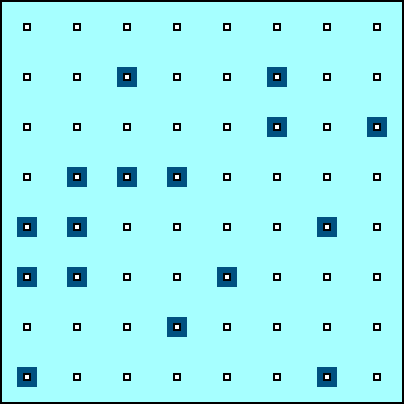
\includegraphics[width=0.23\textwidth]{Images/Sampling_SRS.png}\qquad
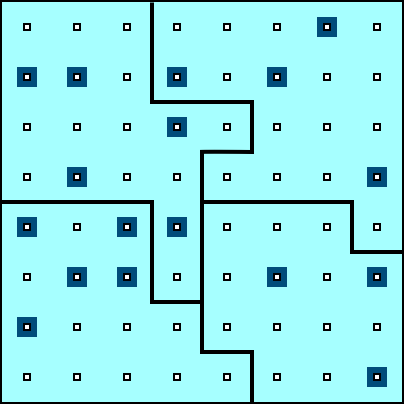
\includegraphics[width=0.23\textwidth]{Images/Sampling_StS.png}\qquad
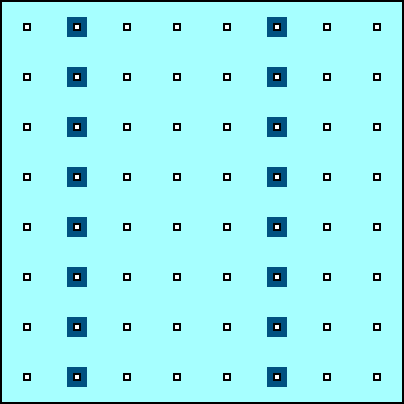
\includegraphics[width=0.23\textwidth]{Images/Sampling_SyS.png}
\\ \ \\
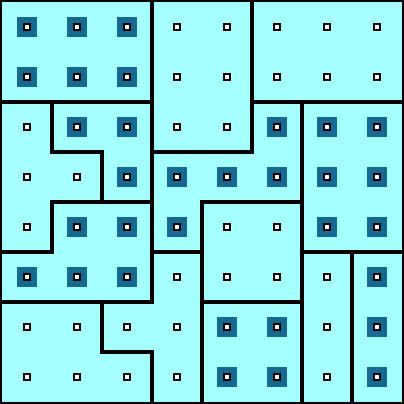
\includegraphics[width=0.23\textwidth]{Images/Sampling_ClS.png}\qquad
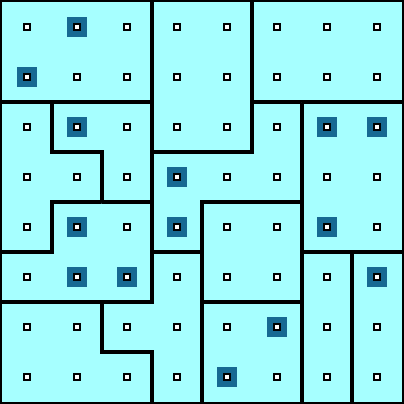
\includegraphics[width=0.23\textwidth]{Images/Sampling_MSS.png}\qquad
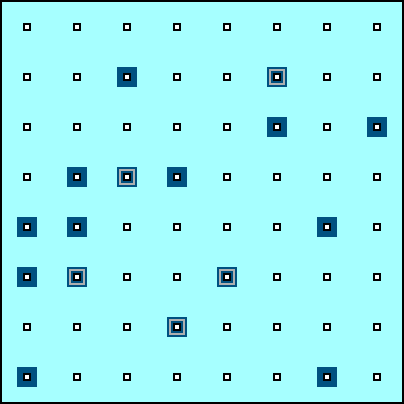
\includegraphics[width=0.23\textwidth]{Images/Sampling_MPS.png}
\caption[\small Schematics of sampling designs]{\small Schematics of sampling designs. Top row, from left to right: simple random sampling, stratified random sampling, systematic random sampling; bottom row, from left to right: cluster sampling, multi-stage sampling, multi-phase sampling.}
\hrule\label{fig:designs}
\end{figure*}
\afterpage{\FloatBarrier}
It is by far the easiest sampling design to implement, and estimates for the resulting sampling errors are well known and easy to compute, which leads to $\SRS$ often being used at a later stage in the sampling process. 
Another advantage is that $\SRS$ does not require auxiliary information, which can be useful with more economical survey frames. \newl This can backfire however, as $\SRS$ makes no use of such information even when it is available. There is also no guarantee that the sample will be representative of the population. Note as well that $\SRS$ may be costly if the sample is widely spread out, geographically.\newl 
The $\SRS$ estimators are 
$$\overline{y}=\frac{1}{n}\sum_{i=1}^n y_i, \quad \hat{\tau}=N\overline{y}, \quad\mbox{and}\quad \hat{p}=\frac{1}{n}\sum_{i=1}^n \delta_i$$ with respective variances
$$\GV(\overline{y})=\frac{\sigma^2}{n}\left(\frac{N-n}{N-1}\right),\quad \GV(\hat{\tau})=N^2\cdot\frac{\sigma^2}{n}\left(\frac{N-n}{N-1}\right),$$ and $$\GV(\hat{p})=\frac{p(1-p)}{n}\left(\frac{N-n}{N-1}\right).$$
The 95\% CI is approximated by substituting the true variance $\sigma^2$ by the unbiased estimator $\frac{n-1}{n}s^2$: $$\hat{\GV}(\overline{y})=\frac{s^2}{n}\left(1-\frac{n}{N}\right), \quad
\hat{\GV}(\hat{\tau})=N^2\cdot\frac{s^2}{n}\left(1-\frac{n}{N}\right),$$ and $$\hat{\GV}(\hat{p})=\frac{\hat{p}(1-\hat{p})}{n-1}\left(1-\frac{n}{N}\right).$$
Finally, the sample size required to achieve an upper error bound $B$ are $$n_{\overline{y}}=\frac{4N\sigma^2}{(N-1)B^2+4\sigma^2},\quad n_{\hat{\tau}}=\frac{4N^3\sigma^2}{(N-1)B^2+4N^2\sigma^2}$$ and $$n_{\hat{p}}=\frac{4Np(1-p)}{(N-1)B^2+4p(1-p)},$$ where $\sigma^2$ and $p$ have been previously estimated (perhaps as part of a prior survey). \newl 
In \textbf{Stratified Random Sampling} ($\StS$), $n=n_1+\cdots+n_k$ units are selected randomly from the survey frame by first establishing $k$ natural strata (such as provinces, or age groups), and selecting $n_j$ units from the $N_j$ units in stratum $j$, with $\overline{y}_j$ and $\hat{p}_j$ the $\SRS$ estimators in stratum $j$, $j=1,\ldots, k$. An illustration is provided in Figure~\ref{fig:designs} (top middle). \newpage\noindent $\StS$ may produce a smaller bound on the error of estimation than would be produced by a $\SRS$ of the same size, particularly if measurements within a strata are homogeneous, and it may be less expensive to implement if the elements are stratified into convenient groupings. Another added benefits is that it may provide parameter estimates for sub-populations that coincide with the strata. There are no major disadvantage to this sample design, except for the fact that there might not be natural ways to stratify the frame (in the sense that each stratum might not be homogeneous in its units), in which case $\StS$ is roughly equivalent to $\SRS$. \newl The $\StS$ estimators are 
$$\overline{y}_{\textrm{st}}=\sum_{j=1}^k \frac{N_j}{N}\overline{y}_j, \quad \hat{\tau}_{\textrm{st}}=N\overline{y}_{\textrm{st}}, \quad\mbox{and}\quad \hat{p}_{\textrm{st}}=\sum_{j=1}^k \frac{N_j}{N}\hat{p}_j,$$ with approximate variances given by 
$$\hat{\GV}(\overline{y}_{\textrm{st}})=\frac{1}{N^2}\sum_{j=1}^kN_i^2\hat{\GV}\left(\overline{y}_j\right),\quad \hat{\GV}(\hat{\tau}_{\textrm{st}})=N^2\hat{\GV}(\overline{y}_{\textrm{st}}),$$ and $$\hat{\GV}(\hat{p}_{\textrm{st}})=\frac{1}{N^2}\sum_{j=1}^kN_i^2\hat{\GV}\left(\overline{p}_j\right).$$
In the $\StS$ design, the sample determination question is two-fold: what size $n$ should the sample have, and how should they be allocated to each stratum ($n_j$, $j=1,\ldots,k$). \par We can select $n$ based on \textbf{cost} considerations or on error bound considerations. Let $c_0$ be the fixed survey operation costs (\textbf{overhead}), $c_j$ be the \textbf{cost per response} in  stratum $j$ (which may need to include the cost of trying to reach non-respondents), and $C$ be the \textbf{total cost} of conducting the survey. The sample size $n$ that minimises  $\hat{\GV}(\overline{y}_{\mbox{st}})$ subject to   $C=c_0+\sum_{j=1}^kc_jn_j$ and $n=\sum_{j=1}^kn_j$ is $$n_{\textrm{st},C}=(C-c_0)\frac{\sum_{j=1}^k \frac{N_j\sigma_j}{\sqrt{c_j}}}{\sum_{j=1}^k N_j\sigma_j\sqrt{c_j}}.$$ In the \textbf{general optimum allocation scheme}, the sampling weights (by strata) are $$w_j=\frac{n_j}{n}=\frac{N_j\sigma_jc_{j}^{-1/2}}{\sum_{\ell=1}^kN_{\ell}\sigma_{\ell}c_{\ell}^{-1/2}}.$$ 
In the \textbf{Neyman allocation scheme}, we assume that the cost per response is identical in each stratum, whence 
$$w_{j,N}=\frac{n_j}{n}=\frac{N_j\sigma_j}{\sum_{\ell=1}^kN_{\ell}\sigma_{\ell}},$$ while in the \textbf{proportional allocation scheme} we further assume that $\sigma_j=\sigma$ for all $j$, so that $$w_{j,P}=\frac{n_j}{n}=\frac{N_j}{N}.$$ Other allocation schemes are also sometimes selected, such as the \textbf{square root proportional scheme} which fixes $$w_{j,S}=\frac{N_j^{1/2}}{\sum_{\ell=1}^kN_{\ell}^{1/2}}$$ in order to insure that smaller strata (e.g. provinces with smaller populations, say) are allocated enough observations to produce sub-population estimates. \newl Note that while budgetary considerations need to be considered in practice, the preceding approach does not allow prescribed error bounds, which could prove problematic. The sample size required to achieve an upper error bound $B$ are\small $$n_{\textrm{st},\overline{y}}=\frac{4\sum_{j=1}^k\frac{N_j\sigma_j^2}{w_j}}{N^2B^2+4\sum_{j=1}^kN_j\sigma_j^2},\quad n_{\textrm{st},\hat{\tau}}=\frac{4N^2\sum_{j=1}^k\frac{N_j\sigma_j^2}{w_j}}{N^2B^2+4\sum_{j=1}^kN_j\sigma_j^2},$$ and $$n_{\textrm{st},\hat{p}}=\frac{4\sum_{j=1}^k\frac{N_jp_j(1-p_j)}{w_j}}{N^2B^2+4\sum_{j=1}^kN_jp_j(1-p_j)},$$ \normalsize where $\sigma_j^2$ and $p_j$ have been previously estimated, and a specific allocation scheme  $\{w_j\}$ has already been selected. \newl 
In \textbf{Systematic Sampling} ($\SyS$), $n$ units are selected randomly from the survey frame by first (randomly) selecting a unit $y_1$ among the first $k=\lfloor\frac{N}{n}\rfloor$ units in the frame and s systematically adding every subsequent $k^{\textrm{th}}$ unit to the sample. An illustration is provided in Figure~\ref{fig:designs} (top right). \newl $\SyS$ is typically appropriate when the frame is already \textbf{sorted} along the characteristic of interest in which case it provides greater information by unit cost than $\SRS$. It is simpler to implement than $\SRS$ since only one random number is required, and like $\SRS$, it does not require auxiliary frame information. Depending on the sample size and on how the frame is sorted, $\SyS$ can produce a sample that is more widely spread (and thus perhaps more representative) than $\SRS$, which may help eliminate other sources of bias.\par On the other hand, it can introduce bias when the pattern used for the systematic sample coincides with a pattern in the population, and it makes no use of auxiliary frame information even if such information exists. Furthermore, any advantage in precision over $\SRS$ disappears if the frame is randomly ordered. Embarrassingly, $\SyS$ may lead to a variable sample size if $n$ does not evenly divide $N$; perhaps more importantly, $\SyS$ does not allow for an unbiased estimator of the sampling variance.\newl For all practical purposes, $\SyS$ behaves like $\SRS$ for a random population. In that case, the $\SRS$ variance  formula may provide a decent approximation. 
\par If the frame is \textbf{ordered} along the characteristic of interest, each $\SyS$ sample will contain some of the smaller values as well as some of the larger values, which would not necessarily be the case in a general $\SRS$ sample. This implies that the  $\SyS$ estimators will have smaller variances than the corresponding $\SRS$ estimators, so that the use of the $\SRS$ variance formula produces an overestimate of the true sampling error in that case. \par In a similar vein, a population is \textbf{periodic} if the frame is \textbf{periodic}  along the characteristic of interest, a $\SyS$ sample that hits both the peaks and valleys of a cyclical trend will bring the method more in line with $\SRS$ and allow the use of the $\SRS$ variance formula as a reasonable approximation. To avoid the problem of underestimating the variation, consider changing the random starting point several times.\newl 
If $n$ divides $N$ evenly, then systematic sampling can be viewed as grouping the population into $k=N/n$ strata, and selecting one unit from each stratum. The difference between $\SyS$ and $\StS$ is that only the first unit is picked randomly in $\SyS$ -- all other samples are automatically selected based on the position of the first choice. \par One can also view $\SyS$ as a one-stage cluster sampling (see the next sub-section), where a primary sampling unit is defined as one of the $k=N/n$ possible systematic samples. An $\SRS$ of one unit can then be drawn from these $k$ primary sampling units. The $\SyS$ sample will consist of all of the items in the selected primary sample.
\newl The $\SyS$ estimators are computed exactly as the corresponding $\SRS$ estimators; their variances are given by  
$$\GV(\overline{y}_{\textrm{sys}})=\frac{\sigma^2}{n}[1+(n-1)\rho],\quad  \GV(\hat{\tau}_{\textrm{sys}})=N^2\GV(\overline{y}_{\textrm{sys}}),$$ and $$\GV(\hat{p}_{\textrm{sys}})=\frac{p(1-p)}{n}[1+(n-1)\rho],$$ where $\rho$ is the \textbf{intra-cluster correlation} (which is typically impossible to compute exactly). \newl Other sampling schemes tend to be substantially more complicated (in the sense that the estimators and variance estimates are harder to derive), but the conceptual ideas behind those sampling schemes are still pretty straightforward; if required, in-depth details can be found in \cite{DC_SC}.
\newl \textbf{Cluster Sampling}
 ($\ClS$), for instance is typically used when the data collection cost increases with the ``distance'' separating the element. The population is separated in clusters, and an $\SRS$ of clusters is selected -- all units within a selected clusters are retained in the sample (see Figure~\ref{fig:designs} (bottom left) for an illustration). As an example, to sample individuals in the population without a population frame (which might be hard to come by), it might be easier to obtain a dwelling frame and to start by sampling dwellings (which are the population \textbf{clusters}), and then to select all individuals in the sampled dwellings. $\ClS$ surveys are usually less expensive and less time-consuming to conduct than $\SRS$, and they can be used to show ``regional'' variations, but they will be wasteful if the cluster sizes are too large, and biased if only a few clusters are sampled.  